% -*- mode: LaTeX; coding: utf-8 -*-
% Typeset with: XeLaTeX

\documentclass{beamer}
\mode<presentation>
{
  \usetheme[progressbar=foot,numbering=fraction,background=light]{metropolis} 
  \usecolortheme{default} % or try albatross, beaver, crane, ...
  \usefonttheme{default}  % or try serif, structurebold, ...
  \setbeamertemplate{navigation symbols}{}
  \setbeamertemplate{caption}[numbered]
  %\setbeamertemplate{frame footer}{My custom footer}
}
\centering

\usepackage{graphicx}
\graphicspath{ {./pr2_figures/} }

% Main document
\begin{document}
\title{DeepSite}
\subtitle{Algorithms in Structural Bioinformatics \\ Project progress report 2}
\author{Thomas Pappas}
%\date{4 March 2020}
\maketitle

\begin{frame}{Outline}
  \tableofcontents
\end{frame}

\section{What is the project about?}

\begin{frame}{What is DeepSite?}
  \begin{block}{DeepSite}
    Protein-binding site \emph{predictor} using 3D-convolutional neural networks
    \begin{itemize}
      \item Using DCNN due to an existing database of 7622 proteins from scPDB to train the NN
      \item Superior performance to two other competitive algorithmic strategies
      \item Available online at \url{https://www.playmolecule.com/deepsite/}
    \end{itemize}
  \end{block}
\end{frame}

\begin{frame}{DeepSite Algorithm summary}
  \begin{block}{Algorithm summary}
    \begin{itemize}
      \item Takes as input a protein ID or a PDB file
      \item Translates the molecular structures to 8 grids representing molecular properties
      \begin{itemize}
        \item The 8 grids are basically channels that NNs take as input
      \end{itemize}
      \item Takes $16 \times 16 \times 16$ \AA$^3$ subgrids from the 8 channels as input for the Deep Convolutional Neural Network (DCNN)
      \item Returns a list of predicted points to be binding-sites, along with their success score
    \end{itemize}
  \end{block}
\end{frame}

\begin{frame}{Example of a 6FAT protein}
  \begin{figure}[h]
    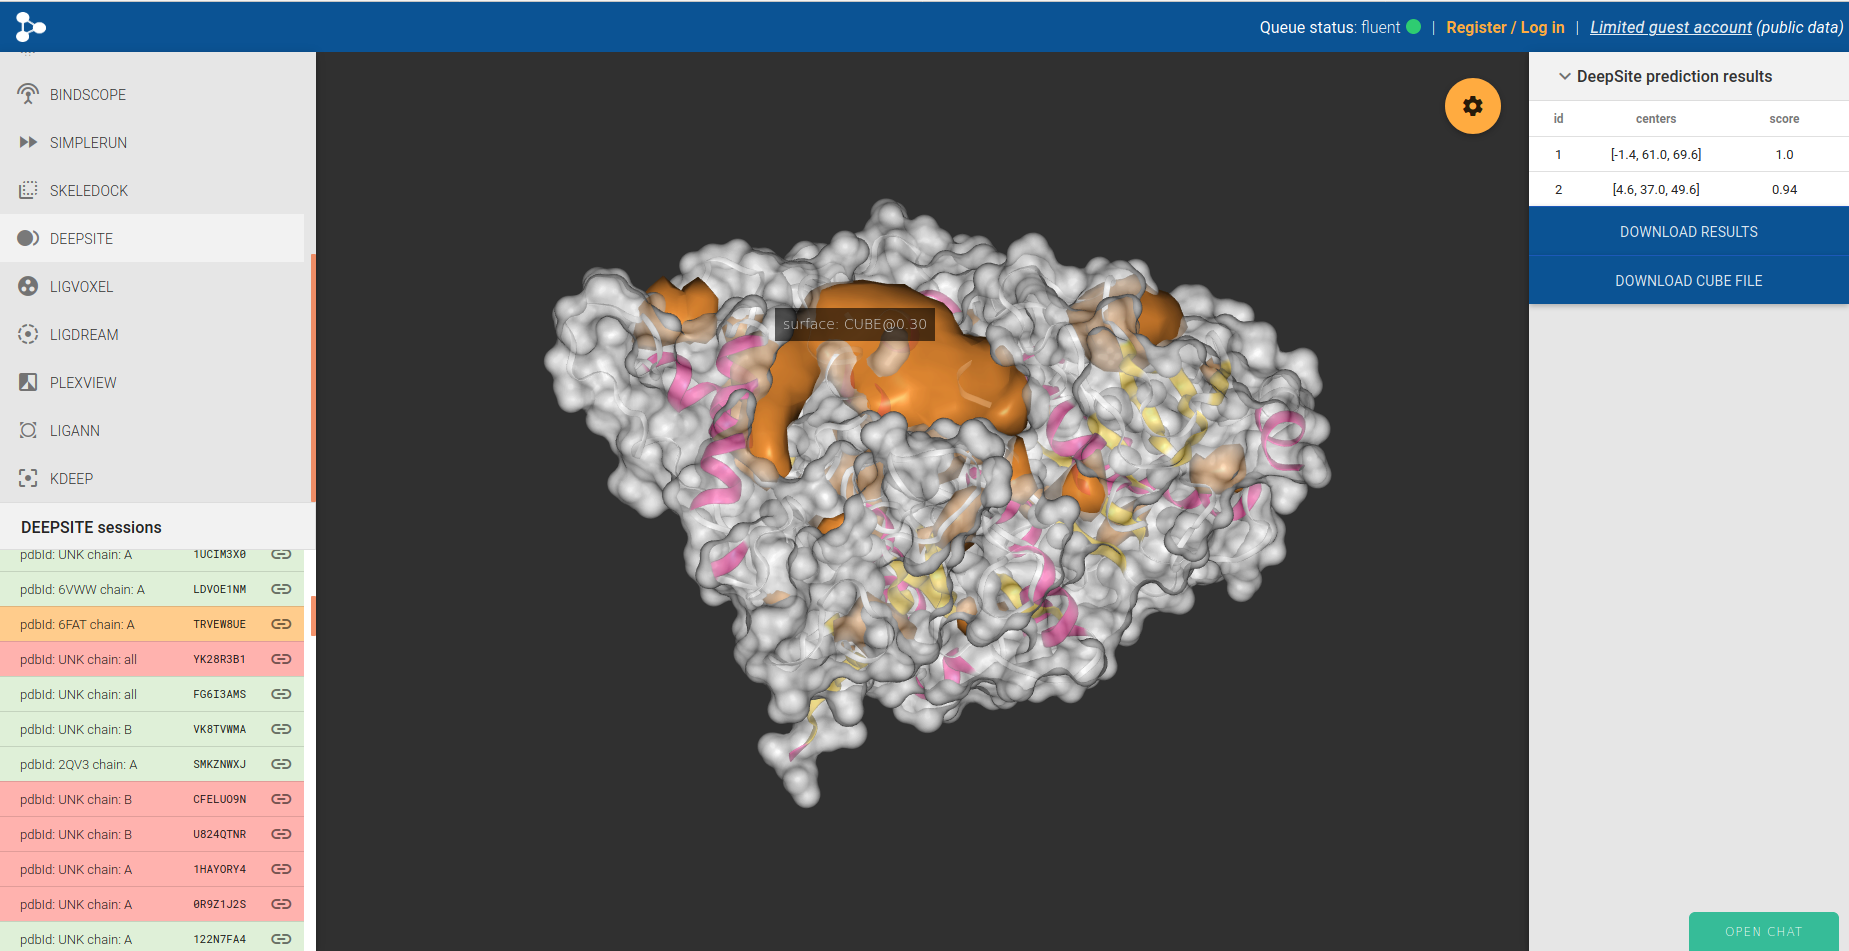
\includegraphics[width=1\textwidth]{deepsite_6fat_result}
    \caption{The 6FAT protein submitted in the \href{https://www.playmolecule.com/deepsite/}{DeepSite web app}}
  \end{figure}
\end{frame}

\section{Translating PDB to NN channels}

\begin{frame}{Translating PDB to NN channels}
  \begin{block}{Parsing the PDB data}
    \begin{itemize}
      \item Parse the atom coordinates from the PDB data
      \begin{itemize}
        \item Use of the HTMDs (Doerr et al., 2016) Python package
      \end{itemize}
      \item Use the AutoDock 4 tables (Tables \ref{table:1} \& \ref{table:2}) and create 8 \emph{filtered set of atoms}, one for each protein property
      \item Consider the space grid containing the protein
      \begin{itemize}
        \item Grid is split to $1 \times 1 \times 1 $ \AA$^3$ voxels
        \item $+8$\AA \;for the cases where the binding pockets are on the edge
      \end{itemize}
    \end{itemize}
  \end{block}
\end{frame}

\begin{frame}{AutoDock 4 tables}
  \begin{columns}
    \begin{column}{.4\textwidth}
      \begin{tiny}
      \begin{table}
      \caption{Atom types}
      \label{table:1}
      \begin{tabular}{ l l }
        \hline
        Element & Description \\
        \hline
        C & Non H-bonding aliphatic carbon \\
        A & Non H-bonding aromatic carbon \\
        NA & Acceptor 1 H-bond nitrogen \\
        NS & Acceptor S Spherical nitrogen \\
        OA & Acceptor 2 H-bonds oxygen \\
        OS & Acceptor S Spherical oxygen \\
        SA & Acceptor 2 H-bonds sulfur \\
        HD & Donor 1 H-bond hydrogen \\
        HS & Donor S Spherical hydrogen \\
        MG & Non H-bonding magnesium \\
        ZN & Non H-bonding zinc \\
        MN & Non H-bonding manganese \\
        CA & Non H-bonding calcium \\
        FE & Non H-bonding iron \\
        \hline
      \end{tabular}
      \end{table}
      \end{tiny}
    \end{column}
    \begin{column}{.6\textwidth}
      \begin{tiny}
      \begin{table}
      \caption{Property-atom type correspondence}
      \label{table:2}
      \begin{tabular}{ l l }
        \hline
        Property & Rule \\
        \hline
        Hydrophobic & atom type C or A \\
        Aromatic & atom type A \\
        Hydrogen bond acceptor & atom type NA or NS or OA or OS or SA \\
        Hydrogen bond donor & atom type HD or HS with O or N partner \\
        Positive ionizable & atom with positive charge \\
        Negative ionizable & atom with negative charge \\
        Metal & atom type MG or ZN or MN or CA or FE \\
        Excluded volume & all atom types \\
      \end{tabular}
      \end{table}
      \end{tiny}
    \end{column}
  \end{columns}
  Table 1, Table 2, 10.1093/bioinformatics/btx350
\end{frame}

\begin{frame}{Translating PDB to NN channels}
  \begin{block}{Atom occupancy}
    We calculate the probability of an atom to exist near the center of a voxel by using the pair correlation function
    \[
      g(r) = exp(-\beta V(r))
    \]
    where $V(r) = \epsilon (r_{vdw}/r)^{12}$ and by taking $\epsilon = \beta^{-1}$ we get the \emph{single atom occupancy estimate} to be
    \[
      n(r) = 1 - exp(-(r_{vdw}/r)^{12})
    \]
  \end{block}
  \begin{block}{Building the NN channels}
    Create a channel (3D matrix) for each of the 8 atom sets, and for each voxel assign the probability of the voxel having an atom of that property (Figure 2)
  \end{block}
\end{frame}

\begin{frame}{Translating PDB to NN channels}
  \begin{figure}[h]
    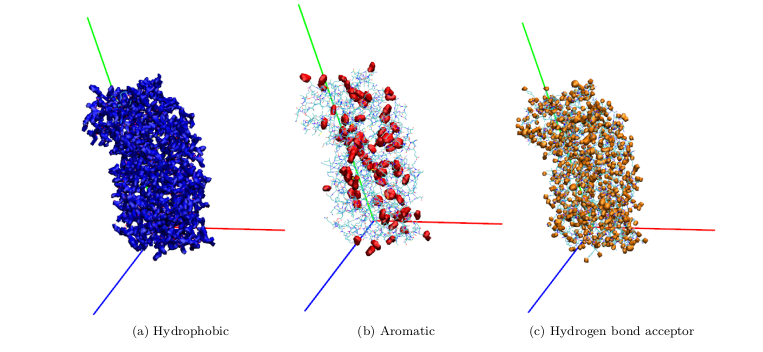
\includegraphics[width=1\textwidth]{deepsite_protein_property_channels}
    \caption{Visual representations of descriptor channels (3/8) for PDB ID 4NIE, Figure S2, 10.1093/bioinformatics/btx350}
  \end{figure}
\end{frame}

\section{NN design}

\begin{frame}{NN design}
  \begin{figure}[h]
    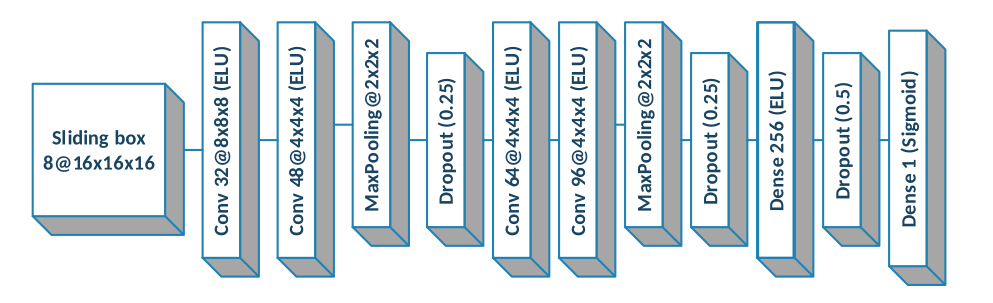
\includegraphics[width=1\textwidth]{deepsite_dcnn_architecture}
    \caption{DeepSite’s internal DCNN architecture, Fig. 2, 10.1093/bioinformatics/btx350}
  \end{figure}
\end{frame}

\begin{frame}{NN design}
  \begin{block}{Training}
    \begin{itemize}
      \item Input subgrids of $16 \times 16 \times 16$ \AA$^3$
      \item Step of 4 voxels
    \end{itemize}
  \end{block}
  \begin{block}{Success criteria for a subgrid}
    Geometric center is closer than 4 Å to the pocket geometric center
  \end{block}
\end{frame}

\section{Evaluating the NN model}

\begin{frame}{10-fold cross-validation}
  Dataset of 7622 scPDB structures
  \begin{block}{Steps}
    \begin{itemize}
      \item Split the training dataset to 10 (equal size) sets
      \item Consider one as a testing set and the rest as training ones and evaluate its success
      \item Cycle through each set and repeat the evaluation
      \item Final result is the average of all above evaluations
    \end{itemize}
  \end{block}
  \begin{block}{Why $k$-fold cross validation?}
    \begin{itemize}
      \item Common practice for validating NN models
      \item Limits the possibility of over-fitting
    \end{itemize}
  \end{block}
\end{frame}

\begin{frame}{Evaluation metrics}
  \begin{block}{Distance to the center of the binding site (DCC)}
    A prediction is successful is closer than a given threshold to the real-binding site
    \begin{itemize}
      \item Values uses range from 4 to 20 \AA
      \item Ignores the shape of the predicted pocket
    \end{itemize}
  \end{block}
  \begin{block}{Discretized volumetric overlap (DVO)}
    Discretize protein space to $1 \times 1 \times 1$ \AA$^3$ voxels and calculate the Jaccard index
    \[
      J = \frac{\#|V_r \cap V_p|}{\#|V_r \cup V_p|}
    \]
    $V_r$: set of voxels in real binding pocket\\
    $V_p$: set of voxels in predicted binding pocket
    \begin{itemize}
      \item Takes into account the shape of the predicted pocket
    \end{itemize}
  \end{block}
\end{frame}

\section{Next Steps}

\begin{frame}{Next Steps}
  \begin{block}{Neural Network design analysis}
  \end{block}
  \begin{block}{Compare results with fPocket and Concavity algorithms}
  \end{block}
\end{frame}

\begin{frame}{Contact details}
  \begin{center}
    Thomas Pappas\\
    \href{mailto:thpappas@di.uoa.gr}{thpappas@di.uoa.gr}
  \end{center}
\end{frame}

\end{document}
